% ---
% titre: Lexique - Qui suis-je ? (feuille élève)
% theme: NO
% chapitre: Nombres naturels et décimaux
% sous_chapitre: 
% niveau: 9e	
% type: JEU
% tags: c-vocabulaire, p-entrainement
% difficulte: 1
% corrige: false
% source: latex
% ---
% NOTE : feuille A4 à photocopier (une par élève). L'élève note le numéro de sa
% fiche en haut, écrit ses trois définitions, puis passe la feuille à un camarade
% qui écrit les mots trouvés dans les cadres. Tags à vérifier contre scripts/tags.md.

% Cadre pour le mot à trouver
\newcommand{\motatrouver}{%
  \begin{tcolorbox}[enhanced, sharp corners, colback=white, colframe=themeColor,
    boxrule=0.6pt, height=1.1cm, valign=center, left=3mm, right=3mm, top=0mm, bottom=0mm]
  \textcolor{themeColor}{\textbf{Mot à trouver}}\,:
  \end{tcolorbox}}

\header{Qui suis-je\,?}
\,\hfill \textbf{Fiche n\textdegree\ \underline{\hspace{1.8cm}}}

\textbf{Auteur\,\textperiodcentered\,e} : \underline{\hspace{5cm}} \hfill
\textbf{Devineur\,\textperiodcentered\,se} : \underline{\hspace{5cm}}

Écris, avec tes propres mots, une définition pour chacun des trois mots de ta fiche, sans écrire le mot (ni un mot de la même famille). Ton camarade devra retrouver chaque mot.

\vfill
\textcolor{themeColor}{\textbf{\large Définition 1}}

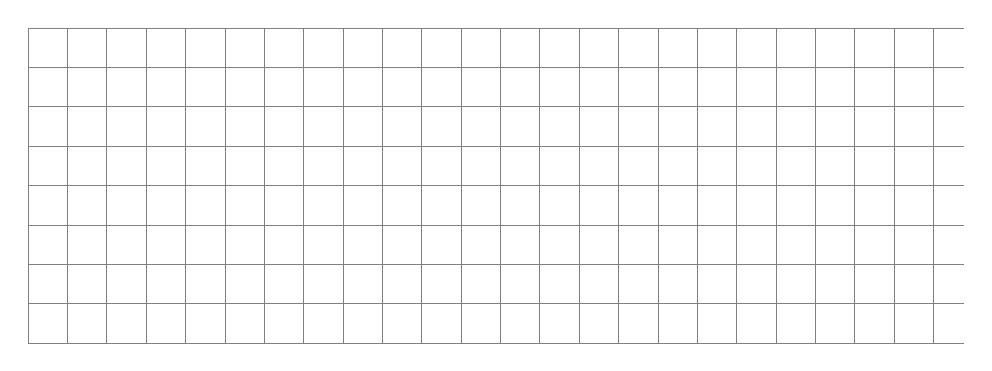
\begin{tikzpicture}\draw[step=0.5cm, gray, very thin] (0,0) grid (0.98\textwidth,4);\end{tikzpicture}
\motatrouver

\vfill
\textcolor{themeColor}{\textbf{\large Définition 2}}

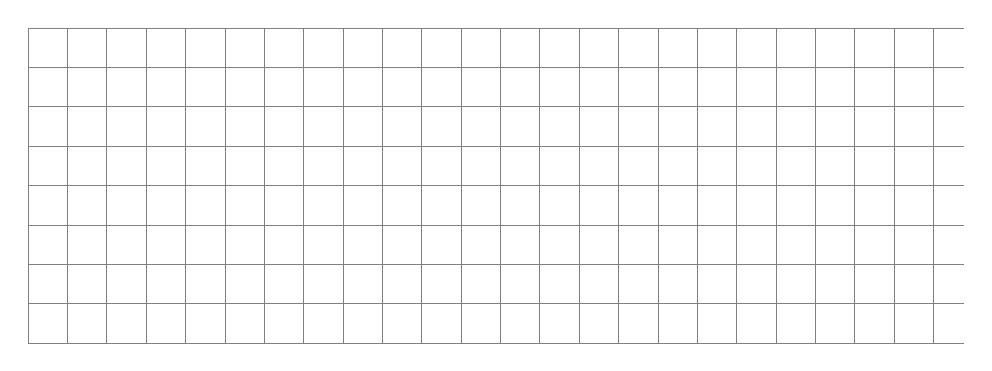
\begin{tikzpicture}\draw[step=0.5cm, gray, very thin] (0,0) grid (0.98\textwidth,4);\end{tikzpicture}
\motatrouver

\vfill
\textcolor{themeColor}{\textbf{\large Définition 3}}

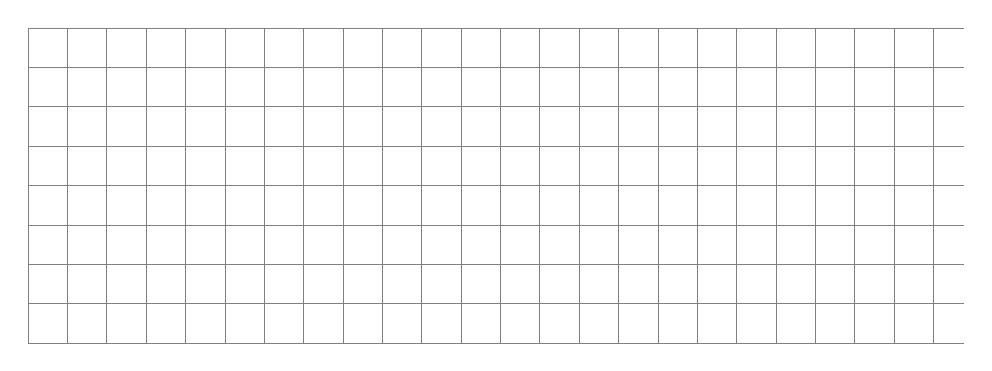
\begin{tikzpicture}\draw[step=0.5cm, gray, very thin] (0,0) grid (0.98\textwidth,4);\end{tikzpicture}
\motatrouver